% CV ----


\documentclass[
  11pt,
]
{article}


% default font
\usepackage{ebgaramond-maths}

\usepackage{iftex}
\ifPDFTeX
  \usepackage[T1]{fontenc}
  \usepackage[utf8]{inputenc}
  \usepackage{textcomp} % provide euro and other symbols
\else % if luatex or xetex
  \usepackage{unicode-math}
  \defaultfontfeatures{Scale=MatchLowercase}
  \defaultfontfeatures[\rmfamily]{Ligatures=TeX,Scale=1}
\fi

% xetex/luatex font selection




% use upquote if available, for straight quotes in verbatim environments
\IfFileExists{upquote.sty}{\usepackage{upquote}}{}
% use microtype if available
\IfFileExists{microtype.sty}{%
\usepackage{microtype}
\UseMicrotypeSet[protrusion]{basicmath} % disable protrusion for tt fonts
}{}
\usepackage[margin=1in]{geometry}





\usepackage{longtable,booktabs}
\usepackage{graphicx,grffile}
\makeatletter
\def\maxwidth{\ifdim\Gin@nat@width>\linewidth\linewidth\else\Gin@nat@width\fi}
\def\maxheight{\ifdim\Gin@nat@height>\textheight\textheight\else\Gin@nat@height\fi}
\makeatother
% Scale images if necessary, so that they will not overflow the page
% margins by default, and it is still possible to overwrite the defaults
% using explicit options in \includegraphics[width, height, ...]{}
\setkeys{Gin}{width=\maxwidth,height=\maxheight,keepaspectratio}



\setlength{\emergencystretch}{3em}  % prevent overfull lines
\providecommand{\tightlist}{%
  \setlength{\itemsep}{0pt}\setlength{\parskip}{0pt}}
\setcounter{secnumdepth}{0}
% Redefines (sub)paragraphs to behave more like sections
\ifx\paragraph\undefined\else
\let\oldparagraph\paragraph
\renewcommand{\paragraph}[1]{\oldparagraph{#1}\mbox{}}
\fi
\ifx\subparagraph\undefined\else
\let\oldsubparagraph\subparagraph
\renewcommand{\subparagraph}[1]{\oldsubparagraph{#1}\mbox{}}
\fi
% TODO: Add custom LaTeX header directives here
\usepackage{graphicx}
\usepackage{fancyhdr}

\pagestyle{fancy}
\fancyhf{}
\renewcommand{\headrulewidth}{0pt}
\fancypagestyle{firstpage}{%
    \fancyhead[R]{%
        \ifnum\value{page}=1%
            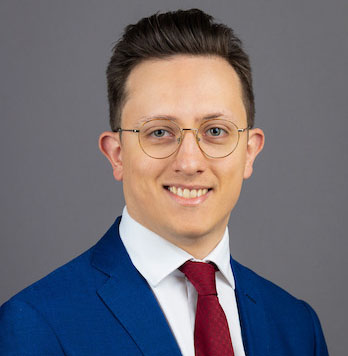
\includegraphics[width = 2 cm]{profile.jpg}%
            \hfill
        \fi
    }
}

\thispagestyle{firstpage}
\makeatletter
\@ifpackageloaded{caption}{}{\usepackage{caption}}
\AtBeginDocument{%
\ifdefined\contentsname
  \renewcommand*\contentsname{Table of contents}
\else
  \newcommand\contentsname{Table of contents}
\fi
\ifdefined\listfigurename
  \renewcommand*\listfigurename{List of Figures}
\else
  \newcommand\listfigurename{List of Figures}
\fi
\ifdefined\listtablename
  \renewcommand*\listtablename{List of Tables}
\else
  \newcommand\listtablename{List of Tables}
\fi
\ifdefined\figurename
  \renewcommand*\figurename{Figure}
\else
  \newcommand\figurename{Figure}
\fi
\ifdefined\tablename
  \renewcommand*\tablename{Table}
\else
  \newcommand\tablename{Table}
\fi
}
\@ifpackageloaded{float}{}{\usepackage{float}}
\floatstyle{ruled}
\@ifundefined{c@chapter}{\newfloat{codelisting}{h}{lop}}{\newfloat{codelisting}{h}{lop}[chapter]}
\floatname{codelisting}{Listing}
\newcommand*\listoflistings{\listof{codelisting}{List of Listings}}
\makeatother
\makeatletter
\makeatother
\makeatletter
\@ifpackageloaded{caption}{}{\usepackage{caption}}
\@ifpackageloaded{subcaption}{}{\usepackage{subcaption}}
\makeatother

% Now begins the stuff that I added.
% ----------------------------------

% Custom section fonts
\usepackage{sectsty}
\sectionfont{\rmfamily\mdseries\large\bf}
\subsectionfont{\rmfamily\mdseries\normalsize\scshape}


% Make lists without bullets
%\renewenvironment{itemize}{
%  \begin{list}{}{
%    \setlength{\leftmargin}{1.5em}
%  }
%}{
%  \end{list}
%}


% Make parskips rather than indent with lists.
\usepackage{parskip}
% \usepackage{titlesec}
% \titlespacing\section{0pt}{12pt plus 4pt minus 2pt}{12pt plus 2pt minus 2pt}
% \titlespacing\subsection{0pt}{12pt plus 4pt minus 2pt}{12pt plus 2pt minus 2pt}

% Use fontawesome. Note: you'll need TeXLive 2015. Update.
%\usepackage{fontawesome5}
\usepackage{fontawesome5}
\newcommand{\custombullet}{\raisebox{0.3ex}{\fontsize{5pt}{5pt}\faCircle}} % Adjust the size here
\renewcommand{\labelitemi}{\custombullet} % Change itemize bullet point style
% Fancyhdr, as I tend to do with these personal documents.
\usepackage{fancyhdr,lastpage}
\pagestyle{fancy}
\renewcommand{\headrulewidth}{0.0pt}
\renewcommand{\footrulewidth}{0.0pt}
\lhead{}
\chead{}
\rhead{}
\lfoot{Giandomenico Bisaccia, MD, PhD}
\cfoot{\apstylekinda\today}
\rfoot{\thepage/{\hypersetup{linkcolor=black}\pageref{LastPage}}}

% Always load hyperref last.
\usepackage{hyperref}
\PassOptionsToPackage{usenames,dvipsnames}{color} % color is loaded by hyperref

\hypersetup{unicode=true,
            pdfauthor={Giandomenico Bisaccia, MD, PhD},
            colorlinks=true,
            linkcolor=blue,
            citecolor=blue,
            urlcolor=blue,
            breaklinks=true, bookmarks=true}
\urlstyle{same}  % don't use monospace font for urls

% Make AP style (kinda) dates for the updated/today field

\usepackage{datetime}
\newdateformat{apstylekinda}{%
  \shortmonthname[\THEMONTH] \THEDAY, \THEYEAR}

% \emph{Updated:} \apstylekinda\today
% ^ removed from that front bar.

\usepackage{orcidlink}
%\usepackage{academicons}
%\definecolor{orcidlogocol}{HTML}{A6CE39}
% \newcommand{\orcid}[1]{\href{https://orcid.org/#1}{\textcolor[HTML]{A6CE39}{\aiOrcid}}}

\usepackage{geometry}

% Set the margins here
\geometry{
    left=1.5cm,
    right=1.5cm,
    top=1.5cm,
    bottom=1.5cm,
}

\begin{document}


\centerline{\huge \bf Giandomenico Bisaccia, MD, PhD}

\vspace{2 mm}

\hrule

\vspace{2 mm}



\centerline{\faEnvelope \hspace{1 mm} \href{mailto:}{\tt bisacciagiandomenico@gmail.com} \hspace{1 mm} }
\centerline{  \faLinkedin \hspace{1 mm} \href{https://www.linkedin.com/in/bisacciamd}{\tt bisacciamd} \hspace{1 mm}  \orcidlink{0000-0003-4606-3093} \hspace{.5 mm} \href{https://orcid.org/0000-0003-4606-3093}{\tt 0000-0003-4606-3093} \hspace{1 mm}  \faLink \hspace{1 mm} \href{http://bisacciamd.com}{\tt bisacciamd.com}  }



\vspace{2 mm}

\hrule



\section{Experience}\label{experience}

\emph{G. d'Annunzio University of Chieti and Pescara, Chieti, Italy}
\hfill May 2024-present

\begin{itemize}
\tightlist
\item
  Research fellow in cardiology

  \begin{itemize}
  \tightlist
  \item
    Supervised clinical research with focus on clinical applications of
    cardiovascular magnetic resonance imaging (CMR)
  \item
    Coordination of undergraduate and postgraduate students
  \end{itemize}
\end{itemize}

\emph{Royal Brompton Hospital, London, UK} \hfill May 2023---present

\begin{itemize}
\tightlist
\item
  Honorary clinical research fellowship (part-time)

  \begin{itemize}
  \tightlist
  \item
    Supervised clinical research on quantitative stress perfusion CMR,
    ischaemic and nonischaemic cardiomyopathies, CMR guidance to
    percutaneous revascularization
  \end{itemize}
\end{itemize}

\emph{Harefield Hospital, London, UK} \hfill Sept 2022---May 2023

\begin{itemize}
\tightlist
\item
  Honorary clinical research fellowship (full time)

  \begin{itemize}
  \tightlist
  \item
    Prepared initial reports for 250+ clinical CMR scans
  \item
    Conducted audit on stress CMR after heart transplantation
  \item
    Researched on CMR in patients with angina, cardiomyopathies, and
    after cardiac transplantation
  \item
    Improved team productivity with coding skills
  \end{itemize}
\end{itemize}

\section{Education}\label{education}

\emph{London School of Economics, London, UK} \hfill Dec 2023---Dec 2025

\begin{itemize}
\tightlist
\item
  MSc in Health Economics, Outcomes and Management in Clinical Sciences
  (class of 2025)

  \begin{itemize}
  \tightlist
  \item
    Taught modules included Economic Analysis for Health Policy
    (distinction), Quality and Outcomes in Clinical Sciences
    (distinction), Economic Evaluation in Health Care, and Fundamentals
    of Management and Leadership (under assessment)
  \item
    Volunteered as the class Clinical Student Representative for 2023/24
  \end{itemize}
\end{itemize}

\emph{Royal Brompton Hospital, London, UK} \hfill Oct---Dec 2022

\begin{itemize}
\tightlist
\item
  Clinical CMR training course

  \begin{itemize}
  \tightlist
  \item
    Underwent full-time training in CMR under Level 3 certified experts
  \item
    Contributed to the CMR service of the hospital
  \end{itemize}
\end{itemize}

\emph{G. d'Annunzio University of Chieti and Pescara, Chieti, Italy}

\begin{itemize}
\tightlist
\item
  PhD (\emph{Doctor Europaeus}) in Neuroscience and Imaging (marked:
  excellent) \hfill Oct 2021---Mar 2024

  \begin{itemize}
  \tightlist
  \item
    Thesis title: \emph{Value of Quantitative Stress Perfusion CMR in
    the Long-Term Assessment of Cardiac Transplantation Recipients}
    (international supervision, revision and examination; PhD defended
    in English)
  \item
    Co-authored 17 peer-reviewed publications
  \item
    Supervised 12 undergraduate and 4 postgraduate students
  \item
    Presented research findings for 7 original research studies at major
    international conferences
  \end{itemize}
\item
  Master's Degree in Medicine (summa cum laude) \hfill Oct 2014---Apr
  2021

  \begin{itemize}
  \tightlist
  \item
    Thesis title: \emph{CMR Reference Values of Mitral and Tricuspid
    Annular Dimensions: the UK BioBank Cohort}
  \item
    MD-PhD research track \hfill Nov 2019-Ott 2020
  \item
    Path of Excellence research track \hfill Ott 2016---Ott 2019
  \end{itemize}
\end{itemize}

\section{Teaching}\label{teaching}

\emph{G. d'Annunzio University of Chieti and Pescara, Chieti, Italy}

\begin{itemize}
\tightlist
\item
  Honorary teaching assistant in clinical applications of CMR,
  Undergraduate radiographer course \hfill May 2024
\end{itemize}

\emph{University of Padua, Italy}

\begin{itemize}
\tightlist
\item
  Lecture on CMR safety, MSc in Cardiac magnetic resonance
  imaging\hfill Jan 2024
\end{itemize}

\section{Professional licenses}\label{professional-licenses}

\begin{itemize}
\tightlist
\item
  Good Clinical Practice certification. \emph{National Institute for
  Health and Care Research}, London, UK \hfill Oct 2022
\item
  UK General Medical Council, reference number 8023039 \hfill Feb 2023
\item
  ``Ordine dei Medici-Chirurghi ed Odontoiatri'', Chieti, Italy, medical
  license number 5690 \hfill May 2021
\end{itemize}

\section{Professional and language
skills}\label{professional-and-language-skills}

\begin{itemize}
\tightlist
\item
  Clinical research

  \begin{itemize}
  \tightlist
  \item
    systematic review and meta-analysis (5 published), diagnostic
    studies (accuracy, clinical utility), prognostic studies (survival
    analysis and modeling)
  \item
    cost-effectiveness analysis and health technology assessment
  \end{itemize}
\item
  Data science and IT

  \begin{itemize}
  \tightlist
  \item
    Strong modelling and data visualization skills in R
  \item
    Dynamic, reproducible reporting in Quarto
  \item
    Development and deployment of server-based Shiny applications
  \item
    Proficient in using Word, Excel, Powerpoint, REDCap and Git, basic
    use of MATLAB, LaTeX, Adobe Illustrator
  \end{itemize}
\item
  English language

  \begin{itemize}
  \tightlist
  \item
    International English Language Testing System (IELTS) \hfill Nov
    2023

    \begin{itemize}
    \tightlist
    \item
      Academic english. Listening 9.0; Reading 9.0; Speaking 8.5;
      Writing 7.5 (scored 1 to 10)
    \end{itemize}
  \item
    Occupational English Test (OET) \hfill Feb 2023

    \begin{itemize}
    \tightlist
    \item
      Medical english. Listening A; Reading A; Speaking B; Writing B
      (scored E to A)
    \end{itemize}
  \end{itemize}
\end{itemize}

\section{Professional affiliations}\label{professional-affiliations}

\begin{itemize}
\item
  \tinyMember of the American Heart Association (2023-present), American
  College of Cardiology (Fellow in Training, 2022-present), Society for
  Cardiovascular Magnetic Resonance (Early Career WG, 2022-present),
  European Society of Cardiology (Professional member, 2021-present),
  European Association of Cardiovascular Imaging (2021-present), and of
  the Italian Society of Cardiology (CMR, Sex differences WG,
  2021-present)
\item
  Other affiliations

  \begin{itemize}
  \tightlist
  \item
    NHS-R Community \hfill 2024-present
  \item
    IMSOGB - Italian Medical Society of Great Britain
    \hfill 2024-present
  \end{itemize}
\end{itemize}

\section{Grants}\label{grants}

\begin{itemize}
\tightlist
\item
  Participant to research unit for the ``ULTRALIGHT-HCM'' study, funded
  by the Italian Ministry of Public Education (PRIN PNRR) for € 299,604
  \hfill July 2023
\end{itemize}

\section{Prizes and awards}\label{prizes-and-awards}

\begin{itemize}
\tightlist
\item
  Finalist, Early career award (clinical track), CMR 2024, London, UK
  \hfill January 2024
\item
  Early Career Investigator Travel Grant, AHA Scientific Sessions,
  Philadelphia, USA \hfill November 2023
\item
  Educational Grant, EACVI Conference, Barcelona, Spain \hfill May 2023
\item
  Travel Grant, SCMR Conference, San Diego, USA \hfill January 2023
\item
  «Path of Excellence» award in Medicine, University of Chieti and
  Pescara, Italy \hfill October 2019
\end{itemize}

\end{document}
